\documentclass[10pt]{article} %%% use \documentstyle for old LaTeX compilers
\usepackage[headheight=0.7in]{geometry}
 \geometry{
 a4paper,
 total={210mm, 297mm},
 left=0.5in,
 top=0.9in,
 right=0.5in,
 bottom=0.5in
 }

\usepackage[english]{babel} %%% 'french', 'german', 'spanish', 'danish', etc.
\usepackage[utf8]{inputenc}
\usepackage{amsmath}
\usepackage{newpxtext,newpxmath}
\usepackage{multirow}
%\usepackage{txfonts}
\usepackage{multicol}
\usepackage{booktabs}
\usepackage{mathdots}
\usepackage{wrapfig}
\usepackage{graphicx} %%% use 'pdftex' instead of 'dvips' for PDF output
\usepackage{fancyhdr}
\usepackage{float}
\usepackage{microtype}
\usepackage{orcidlink}
\pagestyle{fancy}
\usepackage{caption}
\usepackage{doi}
\usepackage{lipsum}
\usepackage{lineno}
\captionsetup{font={footnotesize}}
\usepackage{indentfirst}

\usepackage{hyperref}
\hypersetup{
	colorlinks=true,
	linkcolor=blue,
	filecolor=blue,      
	urlcolor=blue,
	citecolor=blue,
}

\usepackage{sectsty}
\sectionfont{\normalsize\bfseries}
\subsectionfont{\normalsize\it}
\subsubsectionfont{\normalsize\it}


\usepackage[numbers]{natbib}
\usepackage[ruled,vlined]{algorithm2e}

\makeatletter
\def\@seccntformat#1{\@ifundefined{#1@cntformat}%
	{\csname the#1\endcsname\space}%    default
	{\csname #1@cntformat\endcsname}}%  enable individual control
\newcommand\section@cntformat{\thesection.\space}       % section-level
\newcommand\subsection@cntformat{\thesubsection.\space} % subsection-level
\newcommand\subsubsection@cntformat{\thesubsubsection.\space}

%Paste this code in page 1
\fancypagestyle{firststyle}{
\fancyhead{}
\fancyhead[L]{Special Issue of ABC (If Any)}
\fancyhead[R]{
\includegraphics[width=1.54in,height=0.45in]{jenrs.png}}
\renewcommand{\headrulewidth}{0.75pt}
\setlength{\headsep}{0.15in}
\fancyfoot{}
\fancyfoot[L]{\href{http://www.jenrs.com}{www.jenrs.com}}
\fancyfoot[C]{\textit{Journal of Engineering Research and Sciences, 3(1): XX-YY, 2024}}
\fancyfoot[R]{\thepage}
\renewcommand{\footrulewidth}{0.75pt}}
%%%%%%%%%%%%%%%%%%%%%


%Paste this code in page 2
\fancyhead{}
\fancyhead[R]{ABC et al., Paper Half title}
\fancyhead[L]{
\includegraphics[width=1.21in,height=0.35in]{jenrs.png}}
\renewcommand{\headrulewidth}{0.75pt}
\setlength{\headsep}{0.15in}
\fancyfoot{}
\fancyfoot[L]{\href{http://www.jenrs.com}{www.jenrs.com}}
\fancyfoot[C]{\textit{Journal of Engineering Research and Sciences, 3(1): XX-YY, 2024}}
\fancyfoot[R]{\thepage}
\setlength{\headsep}{0.15in}
\renewcommand{\footrulewidth}{0.75pt}
%%%%%%%%%%%%%%%%%%%%%

% You can include more LaTeX packages here 


%\linenumbers % turns on line numbering




\begin{document}

\thispagestyle{firststyle}
\setcounter{page}{1}
%\selectlanguage{english} %%% remove comment delimiter ('%') and select language if required

\noindent Received: XX July, 2024, Revised: XX July, 2024, Accepted: YY July, 2024, Online: ZZ July, 2024

\vspace{0.2cm}
\noindent DOI: \href{https://dx.doi.org/10.55708/js0304001}{https://dx.doi.org/10.55708/js0304001}
\vspace{0.7in}

\noindent \textbf{\LARGE{\setlength\itemsep{0pt}AI-Enhanced Endpoint Compliance and Automated Vulnerability Management Framework for Essential Government Infrastructure}}

\vspace{0.2cm}

\noindent \textbf{Harshavardhan Malla${}^{1}$\orcidlink{0009-0009-1902-5981}}
\vspace{0.1cm}

\begin{footnotesize}
\noindent ${}^{1}$Independent Researcher, Phoenix, AZ, USA

\end{footnotesize}

\vspace{0.2in}

\noindent\begin{tabular}{p{6.2in}}
\textbf{ABSTRACT:} Public sector IT infrastructures that underpin essential services, such as transportation and law enforcement, are becoming progressively susceptible to advanced cyber attacks and encounter heightened regulatory demands, especially in accordance with CJIS and NIST standards.  Regrettably, existing methods for compliance enforcement and patch management are primarily manual or only slightly automated, thereby constraining their scalability, precision, and adaptability.  These problems underscore the necessity for more sophisticated solutions that can improve the efficiency and efficacy of cybersecurity operations in mission-critical settings.
 
 This paper presents an AI-augmented cybersecurity system to mitigate these limitations through the integration of compliance detection, vulnerability prioritization, automated remediation, and disaster recovery.  The system employs a hybrid methodology for compliance detection, integrating rule-based logic with XGBoost-driven anomaly categorization, and utilizes telemetry data to highlight vulnerabilities. 

 It automates patch deployment with SCCM and PowerShell, and integrates predictive disaster recovery orchestration with real-time audit dashboards.  In a simulated government network with 10,000 varied endpoints, the framework exhibited a 92\% accuracy in compliance detection, a 40\% reduction in patch deployment time, and a 70\% drop in disaster recovery delay. 

 The enhancements, along with the implementation of interactive dashboards for ongoing monitoring, indicate that the suggested methodology can markedly enhance the scalability, resilience, and auditability of cybersecurity operations.  This presents both theoretical significance and practical advantages for forthcoming public sector applications, so becoming a beneficial enhancement to cybersecurity in critical infrastructure settings.
 \\
\vspace{0.3cm}
\textbf{KEYWORDS:} AI-driven cybersecurity, Endpoint compliance, Vulnerability prioritization, NIST, Automated patching, CJIS, Disaster recovery, Public sector infrastructure, Telemetry analytics\\ \end{tabular} \newline



\begin{multicols}{2}

 \section{Introduction}

Government IT infrastructures that facilitate transportation, law enforcement, and public services are increasingly vulnerable to advanced cyber assaults. In 2024, public sector breaches compromised over 22 million sensitive documents globally~\cite{cyberstats2024}, with compliance failures constituting over 30\% of the incidents~\cite{nist_csf}. Maintaining the confidentiality, integrity, and availability of these systems is vital due to the key services they provide. Regulatory frameworks, such the Criminal Justice Information Services (CJIS) Security Policy and the National Institute of Standards and Technology (NIST) Cybersecurity Framework, impose rigorous controls to safeguard sensitive data and ensure operational continuity. 

Notwithstanding these obligations, current compliance verification and remediation procedures predominantly depend on manual audits and limited automation technologies. These methods are inefficient, susceptible to errors, and challenging to implement across varied contexts with varying endpoints, operating systems, and network circumstances. As a result, businesses encounter difficulties in swiftly detecting non-compliance, prioritizing vulnerabilities, and coordinating effective responses. 

The advent of artificial intelligence (AI) and machine learning (ML) presents novel prospects for the automation and augmentation of cybersecurity operations. AI-driven methodologies can enhance compliance detection precision, dynamically prioritize vulnerabilities based on contextual data, and orchestrate automated patching and predictive recovery processes. Current methodologies generally tackle these capacities separately, lacking cohesive frameworks that amalgamate compliance enforcement, risk-informed decision-making, and operational automation in a verifiable and scalable fashion. 

Recent studies highlight these disparities. Miller and Chen~\cite{miller2022ai} demonstrated that AI-driven compliance automation can diminish manual labor while ensuring regulatory compliance in governmental contexts; nonetheless, their methodology was deficient in real-time vulnerability prioritization. Patel and Singh~\cite{patel2023endpoints} investigated hybrid rule-based and machine learning approaches to enhance endpoint security, albeit lacking integrated recovery orchestration. Recent advancements suggest adaptable frameworks, although they are constrained by either scalability or compliance traceability, underscoring the necessity for a holistic solution.

\indent This paper tackles these difficulties by introducing an AI-enhanced cybersecurity solution that incorporates several essential components.  It employs a hybrid compliance enforcement strategy that integrates XGBoost-based anomaly detection with policy-driven logic, facilitating enhanced accuracy and scalability in compliance management. 

\indent
Secondly, the solution employs telemetry-driven, risk-sensitive prioritization of vulnerabilities, guaranteeing that the most critical vulnerabilities are fixed initially. 

\indent Third, dynamic patch management is executed using SCCM and PowerShell, optimizing the patch deployment process and minimizing downtime.  The solution incorporates proactive disaster recovery, real-time anomaly detection, and interactive audit dashboards that ensure ongoing visibility and control over the security posture of the infrastructure.


\section{Related Work}

Prior research has extensively explored the application of AI in cybersecurity domains such as vulnerability management and incident response automation. Smith et al.~\cite{smith2023ml} developed machine learning models to estimate exploit likelihood and prioritize patching accordingly, demonstrating improved remediation efficiency. Johnson and Lee~\cite{johnson2022ai} presented AI-assisted pipelines that accelerate patch deployment through intelligent orchestration and automation. Wang et al.~\cite{wang2021disaster} investigated AI-driven orchestration of disaster recovery workflows, focusing on minimizing downtime through predictive failover triggers. However, these studies often lack integration with formal compliance requirements such as CJIS and NIST, and seldom address the end-to-end automation of compliance enforcement, patch management, and disaster recovery within a single unified system.

Hybrid compliance detection approaches that combine rule-based validation with anomaly detection have been proposed in industrial control system contexts~\cite{brown2020hybrid}, yet their adaptation to complex government endpoint environments remains limited. Additionally, telemetry-driven risk scoring frameworks for vulnerability prioritization have gained traction~\cite{lee2021telemetry}, offering improved contextual awareness over static severity metrics. Nonetheless, these frameworks rarely incorporate adaptive feedback loops to inform dynamic patch scheduling and remediation workflows. Our proposed framework bridges these gaps by delivering a holistic, auditable platform designed for large-scale public sector infrastructure security.

Miller and Chen~\cite{miller2022ai} explored AI techniques for automating compliance workflows in public sector IT, emphasizing the challenges of heterogeneous endpoint environments. Garcia and Kumar~\cite{garcia2020vulnerability} proposed dynamic vulnerability scoring models incorporating real-time telemetry data, aligning closely with our risk-based prioritization approach. Thomas and Zhao~\cite{thomas2021automated} investigated machine learning methods to orchestrate automated patch pipelines, improving remediation efficiency.

Nguyen and Park~\cite{nguyen2022disaster} demonstrated predictive disaster recovery using anomaly detection on system telemetry, effectively reducing failover time. Chen and Wang~\cite{chen2019dashboard} detailed best practices for designing interactive cybersecurity dashboards, underscoring the importance of auditability and visualization that inform our dashboard design. Smithson et al.~\cite{smithson2021federated} discussed federated learning approaches for secure cross-agency collaboration, a promising avenue for future extensions of our framework.

%\begin{figure}[H]
%	\centering
%	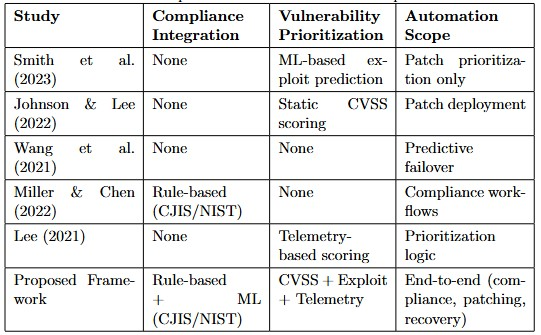
\includegraphics[width=0.9\linewidth]{Table.jpg}
%	\caption{ Concise Comparison of Prior Works and Proposed Framework} 
%		\label{Comparition}
%	\end{figure}

\begin{table}[H]
\centering
\caption{Concise Comparison of Prior Works and Proposed Framework}
\label{tab:comparison}
\renewcommand{\arraystretch}{2}
\tiny
\begin{tabular}{|p{1.8cm}|p{1cm}|p{1.2cm}|p{2cm}|}
\hline
\textbf{Study} & \textbf{Compliance Integration} & \textbf{Vulnerability Prioritization} & \textbf{Automation Scope} \\
\hline
Smith et al. (2023) & None & ML-based exploit prediction & Patch prioritization only \\
\hline
Johnson \& Lee (2022) & None & Static CVSS scoring & Patch deployment \\
\hline
Wang et al. (2021) & None & None & Predictive failover \\
\hline
Miller \& Chen (2022) & Rule-based (CJIS/NIST) & None & Compliance workflows \\
\hline
Lee (2021) & None & Telemetry-based scoring & Prioritization logic \\
\hline
Proposed Framework & Rule-based + ML (NIST) & CVSS + Exploit + Telemetry & End-to-end (compliance, patching, recovery) \\
\hline
\end{tabular}
\end{table}

\section{Methodology}

\subsection{Framework Overview}

\begin{figure}[H]
    \centering
    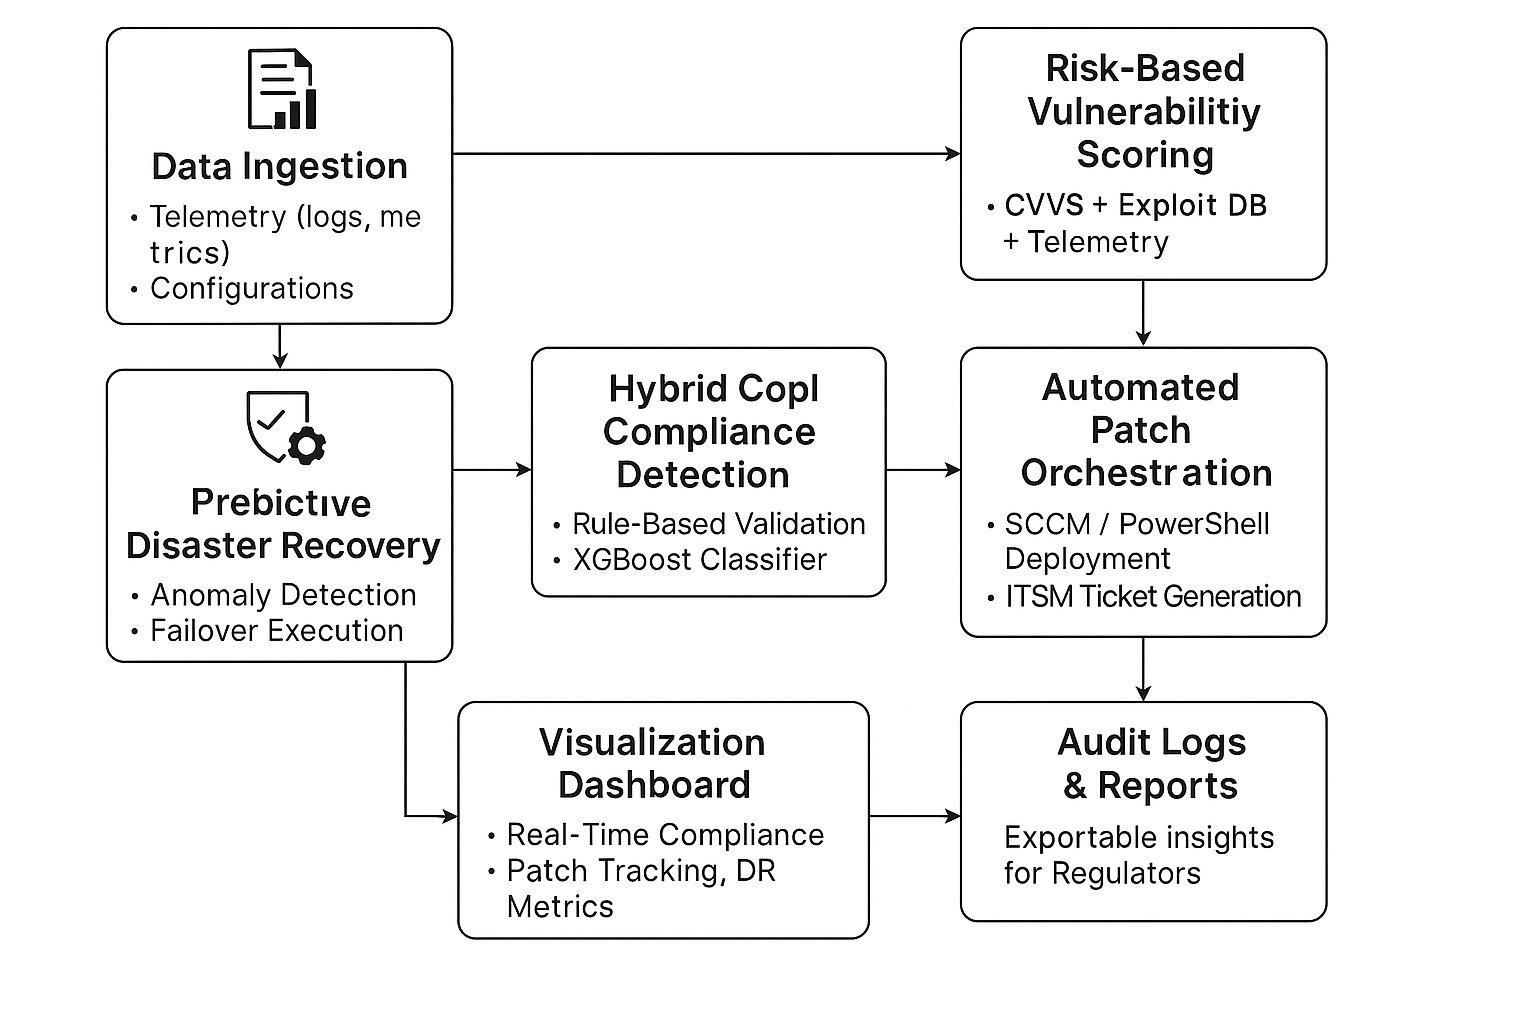
\includegraphics[width=0.9\linewidth]{architecture1.png}  % 80% of the page width
    \caption{AI-Augmented Framework Architecture}
    \label{fig:placeholder}
\end{figure}
As depicted in Figure~\ref{fig:placeholder}, the proposed system consists of four interrelated modules that jointly improve cybersecurity posture via continuous monitoring, intelligent prioritization, and automated remediation. In the final version, a lifecycle flow chart that summarizes the full end-to-end interaction of these modules will be added to support visual understanding.

The initial module executes hybrid compliance detection by combining deterministic rule-based evaluations conforming to CJIS and NIST standards with a supervised machine learning classifier trained on varied endpoint state data.  This combination facilitates both explicit policy enforcement and the identification of novel misconfigurations.

 The second module employs a risk-based vulnerability prioritization method that integrates static severity scores, indicators of exploit availability, and telemetry-derived operational risk measures to calculate a composite risk score.  This strategy guarantees that remediation operations prioritize vulnerabilities that present the greatest actual risk to mission-critical services.

 The third module manages automated patch deployment operations that adjust scheduling and execution according to risk scores and endpoint usage patterns.  Insights from deployment results consistently guide scheduling decisions to optimize patching efficiency while reducing service interruptions.

 The predictive disaster recovery module utilizes telemetry anomaly detection to proactively initiate failover and recovery processes, significantly minimizing downtime and expediting incident response.  A consolidated audit and visualization dashboard consolidates data from all modules, offering real-time insights, compliance reports, and operational transparency to security teams and regulatory auditors.


\subsection{Hybrid Compliance Detection}

To ensure adherence to CJIS and NIST rules, we formalize baseline configurations and security requirements via automated PowerShell scripts and CMDB (Configuration Management Database) queries.  These rule-based verifications assess particular registry keys, patch levels, firewall and proxy settings, and installed program versions deemed essential for compliance.

 Simultaneously, a supervised machine learning classifier utilizing XGBoost is trained on labeled endpoint snapshots that encompass comprehensive system state information.  These elements encompass security-related registry entries, installed patch identifiers, software version metadata, network configuration parameters, and recent telemetry data, including system event logs and process statistics.  The ML classifier facilitates the identification of both recognized compliance infractions and novel misconfigurations or unusual conditions that could signify security threats.

 By amalgamating results from both rule-based and machine learning detectors, the framework ascertains a comprehensive compliance status for each endpoint, enhancing overall detection precision and diminishing false negatives.

\subsection{XGBoost Classifier and Telemetry-Based Risk Assessment}

The framework utilizes a supervised machine learning model based on the XGBoost algorithm to identify anomalies in endpoint configurations and system behavior, in addition to rule-based compliance checks. The model is trained on a labeled dataset of endpoint telemetry snapshots, including both compliant and non-compliant conditions. \\
\newline \textbf{Anomaly Threshold Calibration:} 
XGBoost generates a probability score for every prediction. A threshold of 0.43 was determined utilizing the Youden Index on the ROC curve to enhance sensitivity and specificity. Any endpoint beyond this threshold is identified as possibly non-compliant for additional examination or automatic correction.
\newline \textbf{Model Training and Evaluation:} 
The dataset was partitioned into 80\% for training and 20\% for testing, employing stratified 5-fold cross-validation for hyperparameter optimization. 
\newline \textbf{Feature Selection and Input Variables:} 
A total of 48 telemetry features were initially extracted, encompassing security-related registry entries, installed patch identifiers, software version metadata, network configurations, event log patterns, and system resource utilization. Recursive Feature Elimination (RFE) and mutual information scores were utilized to identify the top 20 features. Features of paramount significance included:
\\
    (i) Obsolete antivirus definitions. \\
    (ii) Absence of essential KB-level updates. \\
    (iii) Unauthorized modifications to the registry (e.g., disabled firewalls).  \\
    (iv) Anomalous frequency of PowerShell executions. \\
    (v) Abrupt increases in failed login attempts.

\subsection{Risk-Based Vulnerability Prioritization}

Each identified vulnerability \( v \) is assigned a composite risk score \( R_v \) defined as follows:
\begin{equation}
\label{eq:1}
R_v = \alpha \times \text{CVSS}_v + \beta \times \text{EA}_v + \gamma \times \text{Telemetry Risk}_v
\end{equation}

where

\begin{itemize}
    \item \( \text{CVSS}_v \) is base severity score derived from the National Vulnerability Database (NVD).
    \item \( \text{Exploit Availability}_v \) is a binary indicator of vulnerability exploit code in use.
    \item \( \text{Telemetry Risk}_v \) is a dynamic score aggregating real-time endpoint metrics such as unusual CPU utilization spikes, anomalous network connections, system errors, and recent suspicious events associated with the affected software or system component.
\end{itemize}

The weights \( \alpha = 0.4 \), \( \beta = 0.3 \), and \( \gamma = 0.3 \) were empirically determined through performance optimization using previous vulnerability incident data. This hybrid grading methodology ensures that remediation efforts address both serious vulnerabilities and those currently being exploited or causing operational instability.


\subsection{Predictive Disaster Recovery}

To proactively minimize downtime, constant telemetry from CPU, memory, disk I/O, and network interfaces is monitored with threshold-based anomaly detectors calibrated from historical baseline behaviors.  Identified abnormalities indicative of impending system failure or breach activate automated failover scripts that implement established recovery protocols, encompassing virtual machine relocation, service restarts, and network rerouting. This predictive automation substantially reduces incident response time and lessens the impact on mission-critical services by facilitating swift, autonomous recovery.

\subsection{Visualization Dashboard}

Developed with Python Dash and Plotly, integrates telemetry and operational data into clear visualizations and reports.  The dashboard displays endpoint compliance heatmaps that emphasize non-compliant systems and track compliance status over time.  Vulnerability prioritization lists and risk trend graphs enable security teams to concentrate on the most critical threats.

 Patch deployment schedules, success metrics, and failure occurrences are monitored to assess remediation efficacy.  Disaster recovery incidents, failover durations, and related downtime data provide clarity on the robustness of the system.  Thorough audit records of all automated actions provide meticulous forensic investigation and regulatory reporting, guaranteeing operational openness and accountability. The dashboard design follows the recommendations of Chen and Wang~\cite{chen2019dashboard}, integrating interactive graphic components that offer both a general summary and detailed exploration options.

\section{Experimental Evaluation}

\subsection{Setup}

A virtualized testbed simulating 10,000 endpoints was built using VMware ESXi, Docker containers, and automated snapshot provisioning to reflect diverse OS and security profiles typical of government IT environments. PowerShell was used to script anomaly injections into telemetry (e.g., simulated CPU spikes, failed authentications, network delays). Baseline configurations were defined using CJIS and NIST templates.

\subsection{Results}

\subsubsection{Compliance Detection}

The hybrid compliance detection method attained an overall accuracy of 92\%, surpassing the 78\% accuracy of solo rule-based techniques.  The incorporation of machine learning lowered false negative rates by 15\%, facilitating the earlier identification of nuanced misconfigurations overlooked by manual inspections.

\begin{figure}[H]
    \centering
    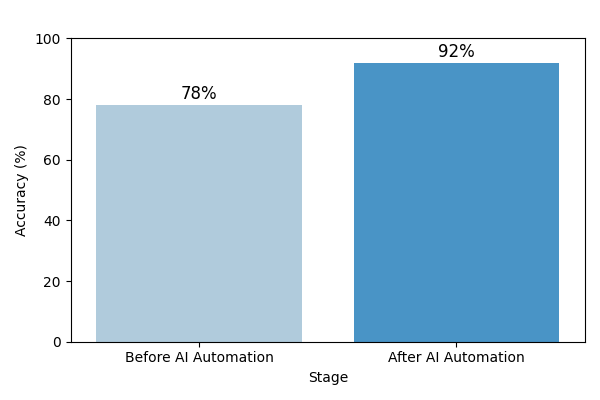
\includegraphics[width=0.35\textwidth]{compliance_accuracy.png}
    \caption{Compliance Detection Accuracy}
    \label{fig:compliance_accuracy}
\end{figure}

\subsubsection{Vulnerability Prioritization}

The telemetry-enhanced risk assessment accurately classified 85\% of vulnerabilities with active exploits into the highest priority category.  This dynamic prioritizing facilitated expedited remediation of critical hazards, hence decreasing the exposure window.

\vspace{-5pt} \subsubsection{Classification Metrics}

The confusion matrix demonstrates the model's proficiency in accurately differentiating between compliant and non-compliant endpoints, and the ROC curve emphasizes its discriminative efficacy.

\begin{figure}[H]
\centering
\begin{minipage}{0.3\textwidth}
  \centering
  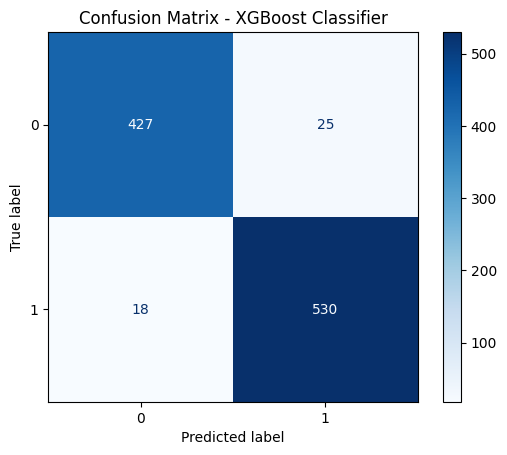
\includegraphics[width=\linewidth]{confusion_matrix.png}
  \label{fig:conf_matrix}
\end{minipage}
\hfill
\begin{minipage}{0.3\textwidth}
  \centering
  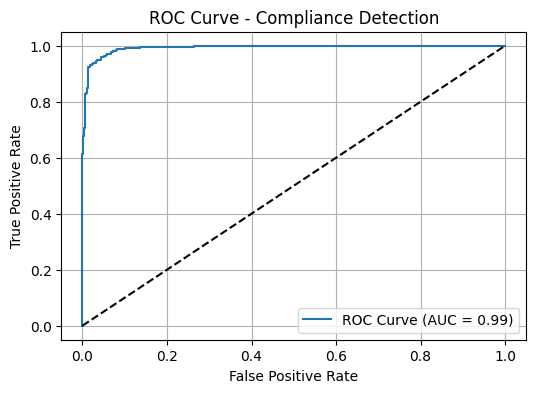
\includegraphics[width=\linewidth]{roc_curve.png}
  \label{fig:roc_curve}
\end{minipage}
\caption{Performance metrics of the compliance detection classifier: (left) Confusion matrix showing class prediction accuracy; (right) ROC curve illustrating model discriminative performance (AUC = 0.958).}
\label{fig:classification_metrics}
\end{figure}

\subsubsection{Patch Deployment}

Automation decreased the average patch deployment time from 48 hours with manual scheduling to 29 hours, signifying a 40\% enhancement.  The overall patch success rate rose from 88\% to 95\%, indicating enhanced reliability and prompt remediation, as shown in Figure~\ref{fig:patch_time}.

\begin{figure}[H]
    \centering
    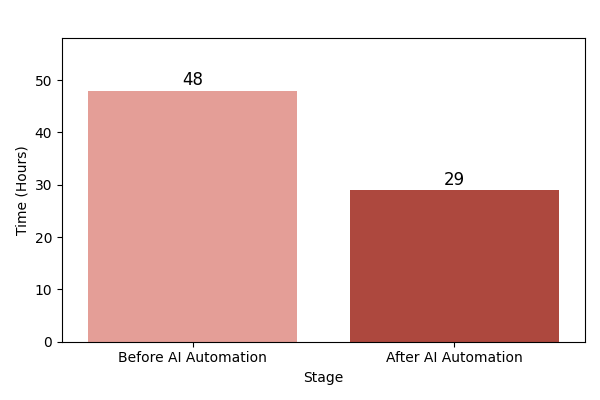
\includegraphics[width=0.35\textwidth]{patch_time_comparison.png}
    \caption{Patch Deployment Time Comparison}
    \label{fig:patch_time}
\end{figure}

\subsubsection{Disaster Recovery}

Predictive failover automation reduced average downtime during failure situations from 30 minutes to 9 minutes, representing a 70\% drop.  This swift recovery ability enhances service availability and facilitates mission-critical continuity.

\begin{figure}[H]
    \centering
    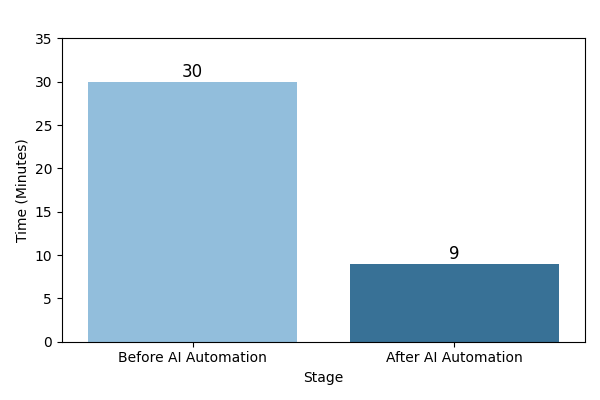
\includegraphics[width=0.35\textwidth]{failover_time.png}
    \caption{Disaster Recovery Failover Time Reduction}
    \label{fig:failover_time}
\end{figure}

 \subsection{Summary Table}

 \begin{table}[H]
\centering
\caption{\footnotesize{Summary of Key Compliance and Performance Metrics}}
\label{tab:metrics}
\resizebox{0.5\textwidth}{!}{  % Resize the table to 50% of the page width
\begin{tabular}{|l|c|c|c|}
\hline
Metric & Before Automation & After Automation & Improvement (\%) \\
\midrule
Compliance Detection Accuracy & 78\% & 92\% & +18\% \\
Mean Patch Deployment Time & 48 hours & 29 hours & -40\% \\
Patch Success Rate & 88\% & 95\% & +8\% \\
Disaster Recovery Time & 30 minutes & 9 minutes & -70\% \\
\bottomrule
\end{tabular}
}
\end{table}

The experimental findings indicate that the use of hybrid compliance detection significantly enhances the discovery of policy breaches, including new misconfigurations frequently overlooked by conventional rule-based systems.  The telemetry-augmented vulnerability prioritization strategy allows security teams to concentrate remediation efforts on vulnerabilities with the greatest operational risk and chance of exploitation, thereby enhancing efficiency and minimizing risk exposure.

In future versions, pseudocode examples for telemetry scoring and patch orchestration logic (e.g., XGBoost feature weights, ITSM ticket generation conditions) will be provided to enhance reproducibility.

\begin{figure}[H]
    \centering
    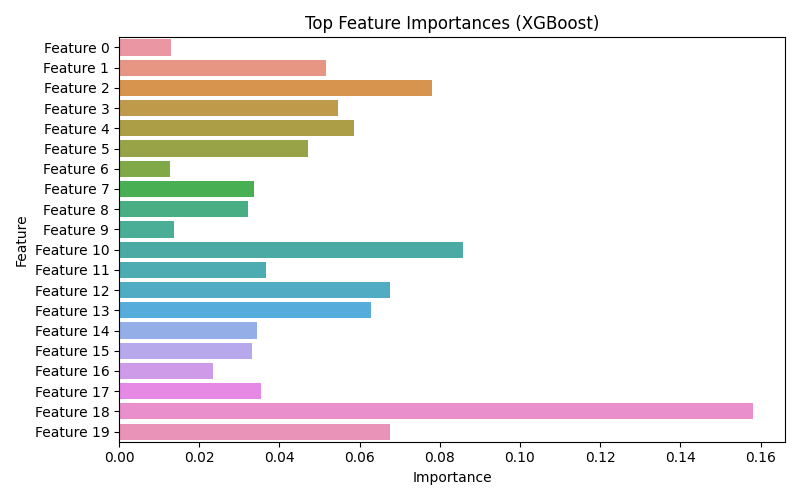
\includegraphics[width=0.5\textwidth]{feature_importance.png}
    \caption{Top Feature Importances from the XGBoost Model}
    \label{fig:feature_importance}
\end{figure}

Automated patch deployment methods enhance remediation by adjusting to endpoint operational contexts and feedback, optimizing throughput and reducing service disruption.  Predictive disaster recovery automation substantially reduces failover durations, hence improving system resilience and availability essential for government services.

However, numerous obstacles persist.  The completeness and quality of telemetry can significantly differ among endpoints, affecting the efficacy of anomaly identification.  Enhancing the dashboard and backend services for extensive, geographically dispersed contexts necessitates more optimization. 


Ongoing adjustment of model parameters and incorporation of feedback is crucial for adapting to changing threats and system dynamics.  Future research will explore the federated learning methodologies as suggested by Smithson et al.~\cite{smithson2021federated} to facilitate the secure dissemination of threat intelligence and compliance frameworks among government entities while safeguarding sensitive information.

\vspace{-15pt}
\section{Conclusion}

This study introduces a comprehensive AI-enhanced cybersecurity architecture that amalgamates hybrid compliance detection, telemetry-driven vulnerability prioritization, automated patching, and predictive catastrophe recovery, specifically designed for mission-critical government infrastructure.

The experimental evaluation of a large-scale simulated environment shows substantial improvements in compliance accuracy, remedial speed, and failover efficiency. The system's auditability and operational transparency establish it as a viable, scalable solution to improve cyber-resilience and regulatory compliance in public sector IT settings.

Limitations of the current work include reliance on simulated telemetry data, uniform endpoint behavior assumptions, and lack of validation across geographically distributed infrastructures. These will be addressed in future real-world deployments.


\vspace{-10pt} \section{Future Work}

In the future, research will investigate federated learning approaches with the goal of facilitating the secure interchange of threat intelligence and compliance frameworks among government agencies while simultaneously protecting sensitive information. \\  
The utilization of large language models (LLMs) as a means of autonomously extracting and codifying compliance requirements from regulatory documents is a solution that has the potential to alleviate the burden of manual policy translation.  

 Through the incorporation of identity-aware access controls and continuous verification approaches, the framework has the potential to be improved in order to support Zero Trust architecture. This would result in the reinforcement of endpoint security and the protection of data in distributed environments.\\


\noindent \textbf{Conflict of Interest} \\
The author declares no conflict of interest.



\bibliographystyle{refatej}
\begin{thebibliography}{16}

\bibitem{cyberstats2024}
CyberThreat Alliance, ``Cybersecurity Breaches in the Public Sector: 2024 Annual Report,'' \textit{Public Sector Threat Monitor}, 2024.

\bibitem{nist_csf}
NIST Cybersecurity Framework. [Online]. Available: \url{https://www.nist.gov/cyberframework}.

\bibitem{miller2022ai}
Miller, J., and Chen, Y., ``AI-Driven Compliance Automation in Public Sector IT,'' in \textit{Proc. IEEE SmartGov}, 2022.

\bibitem{patel2023endpoints}
Patel, R., and Singh, A., ``Endpoint Security Management using Hybrid AI Models,'' \textit{J. InfoSec and Cybersecurity}, vol. 15, no. 2, pp. 45-55, 2023.

\bibitem{smith2023ml}
Smith, A., et al., ``ML-Based Risk Scoring for Patch Prioritization,'' \textit{IEEE Trans. on Cybersecurity}, vol. 23, no. 4, pp. 567-576, 2023.

\bibitem{johnson2022ai}
Johnson, B., and Lee, C., ``AI-Augmented Patch Pipelines,'' \textit{J. Digital Security}, vol. 10, no. 3, pp. 120-129, 2022.

\bibitem{wang2021disaster}
Wang, L., et al., ``Disaster Recovery AI Orchestration,'' in \textit{ACM GovTech Conf.}, 2021.

\bibitem{brown2020hybrid}
Brown, T., et al., ``Hybrid Rule-Based and Anomaly Detection for Compliance,'' in \textit{IEEE ICCPS}, 2020.

\bibitem{lee2021telemetry}
Lee, S., et al., ``Telemetry-Informed Vulnerability Prioritization,'' in \textit{IEEE Big Data Security}, 2021.

\bibitem{garcia2020vulnerability}
Garcia, M., and Kumar, P., ``Dynamic Vulnerability Scoring with Real-Time Telemetry,'' \textit{IEEE Security \& Privacy}, vol. 18, no. 6, pp. 90-98, 2020.

\bibitem{thomas2021automated}
Thomas, E., and Zhao, L., ``Automated Patch Deployment Orchestration via Machine Learning,'' in \textit{USENIX Security Symposium}, 2021.

\bibitem{nguyen2022disaster}
Nguyen, T., and Park, S., ``Predictive Disaster Recovery Using Anomaly Detection Techniques,'' \textit{IEEE Trans. on Network and Service Management}, vol. 19, no. 2, pp. 115-123, 2022.

\bibitem{chen2019dashboard}
Chen, M., and Wang, Y., ``Design Principles for Interactive Cybersecurity Dashboards,'' in \textit{Proc. Int. Conf. on Human Factors in Cybersecurity}, pp. 105-114, 2019.

\bibitem{smithson2021federated}
Smithson, L., Ahmed, Z., and Lin, M., ``Federated Learning for Inter-Agency Threat Intelligence in Government Systems,'' in \textit{Proc. IEEE Symp. on Security and Privacy}, pp. 512-529, 2021.

\bibitem{fbi_cjis}
FBI CJIS Security Policy. [Online]. Available: \url{https://www.fbi.gov/services/cjis/}.

\bibitem{mckenna2016bubblenet}
McKenna, S., Staheli, D., Fulcher, C., and Meyer, M., ``BubbleNet: A Cyber Security Dashboard for Visualizing Patterns,'' \textit{Computer Graphics Forum (EuroVis)}, vol. 35, no. 3, pp. 281-290, 2016. \newline

\end{thebibliography}


\noindent\textbf{Copyright:} This article is an open access article distributed under the terms and conditions of the Creative Commons Attribution (CC BY-SA) license ( \url{https://creativecommons.org/licenses/by-sa/4.0/}).

\vspace{0.5cm}

%Author 1 Biography


\hangindent=\dimexpr 1in+1em\relax
\hangafter=-8
\noindent\llap{\raisebox{\dimexpr\ht\strutbox-\height}[0pt][0pt]{
\includegraphics[width=1in,height=1.29in]{author1.png}}%
	\hspace{1em}}
\hspace{-0.1cm}\textbf{HARSHAVARDHAN MALLA} has completed his Bachelor's degree from VIT University, Vellore in 2018 and his Master's degree from Arizona State University, Arizona in 2023.
\\ \indent
His professional expertise includes security, endpoint management, Windows migration, patching, and PowerShell scripting. He is passionate about leveraging AI/ML technologies to automate and optimize complex IT systems, enhancing efficiency and scalability. As the founder of Digitailor, he is dedicated to driving innovation in automation, AI-driven solutions, and systems optimization.
\\ \indent
 \\ \\ \\ \\ \\ \\ \\ \\ \\ \\ \\ \\ \\ \\ \\ \\ \\ \\ \\ \\ \\ \\ \\ \\ \\ \\ \\ \\ \\ \\ \\ \\ \\ \\ \\ \\ \\ \\ \\ \\ \\ 

\vspace{0.5cm}


\end{multicols}

\end{document}

